\documentclass[a0paper,portrait]{tikzposter}
% \usepackage{graphicx}
% \usepackage{tabularx}
% \usepackage{color}
\usepackage{amssymb,amsfonts}
\usepackage{easySymbols}
\usepackage{caption}
% \usepackage[super,sort&compress,comma]{natbib}

\tikzposterlatexaffectionproofoff

\title{Avoiding pitfalls in $L_1$-regularised inference of gene networks}
\institute{\normalsize
  $^{a}$Stockholm Bioinformatics Centre, Science for Life Laboratory, Box 1031, 17121 Solna, Sweden\\
  $^{b}$Department of Biochemistry and Biophysics, Stockholm University\\
  $^{c}$Department of Immunology, Genetics and Pathology, Uppsala University, Rudbeck laboratory, 75185 Uppsala, Sweden\\
  $^{d}$Science for Life Laboratory, Uppsala University\\
  $^{e}$Swedish eScience Research Center}

\author{
  Andreas Tj\"arnberg,\textit{$^{ab}$}
  Torbj\"orn E.~M. Nordling,\textit{$^{acd}$}
  Matthew Studham,\textit{$^{a}$}\\
  Sven Nelander,\textit{$^{cd}$} and
  Erik~L.L.~Sonnhammer,\textit{$^{abe}$}}

% \titlegraphic{Ble}
\usetheme{Board}
% \usecolorstyle{Sweden}
% \usebackgroundstyle{VerticalGradation}
% \usetitlestyle{Empty}
% \useblockstyle{TornOut}
% \usenotestyle{Sticky}

\usecolorpalette{GreenGrayViolet}
% \usebackgroundstyle{VerticalGradation}
% \useinnerblockstyle{Board}


\begin{document}
\maketitle

\begin{columns}
  \column{0.5}
  \block{The Problem}{

    Statistical regularisation methods such as \lasso and related
    $L_1$ regularised regression methods are commonly used to
    construct models of gene regulatory networks.
    \\\\
    Although they theoretically can infer the correct network
    structure under the linear systems approximation assumption,
    they have been shown in practice to make errors, \ie leave out
    existing links and include non-existing links.
    \\\\
    \coloredbox{\centering Linear systems representation
      \begin{equation*}
        \mY = -\mA^{-1}\mP +\mA^{-1}\mF + \mE
        \label{eq:Linearmap}
      \end{equation*}
    }%
    \coloredbox{\centering
      $L_1$ regularisation (\lasso)
      \begin{equation*}
        \hat{\mA}_{\textrm{reg}}(\tilde{\zeta}) = \arg \min_{\mA} ||\bA \bY+\bP||_{L_2}^2 + \tilde{\zeta}||\bA||_{L_1} .
      \end{equation*}
    }
  }

  \column{0.5}
  \block[titleoffsety=-50mm,bodyoffsety=-50mm]{$L_1$ regularisation pitfall}{
    \begin{itemize}
    \item $L_1$ GRN inference methods fail even though the data is
      informative enough for inferring the correct network
      structure.
      \begin{itemize}
      \item Inference methods performance is dependent on data properties
      \item Underlying system structure enforces response patterns
        and defines data properties
      \item Design of experiments dictates final data structure
      \end{itemize}

    \end{itemize}
    

  }
\end{columns}


\begin{columns}

  \column{0.3}
  \block{Data properties}{ % To move block [titleoffsetx=100mm,bodyoffsetx=100mm]
    \innerblock{ill-conditioned response}{
      \begin{tikzfigure}{}
        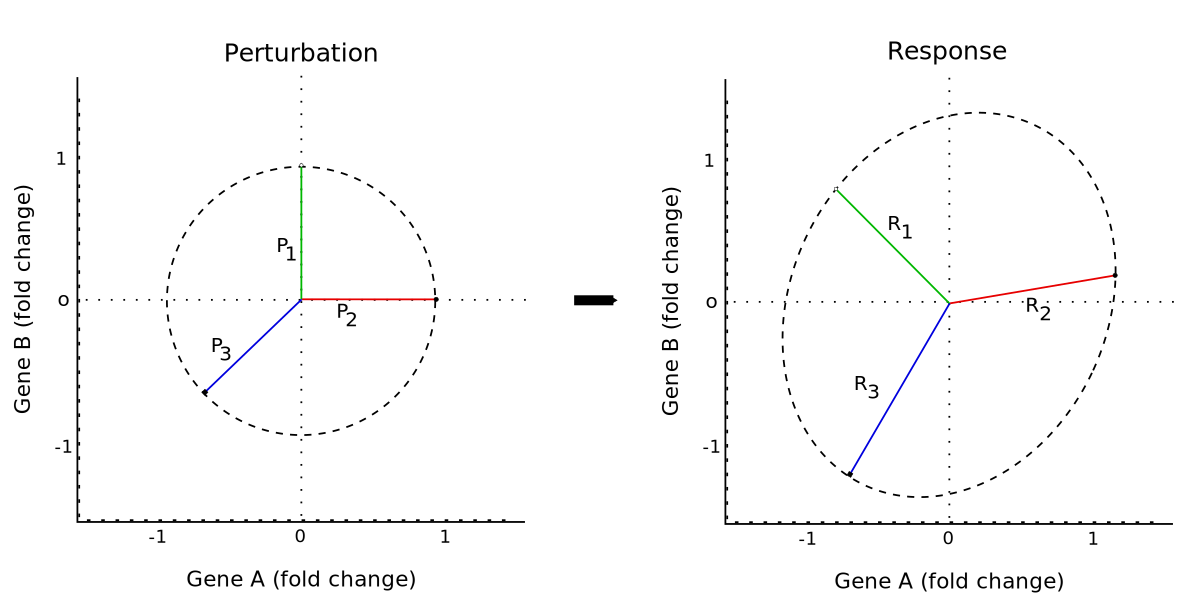
\includegraphics[width=1.0\linewidth]{./img/ill-conditioned-data}
      \end{tikzfigure}
    }
    ~~~~~~
    \innerblock{well-conditioned response}{
      \begin{tikzfigure}{}
        \includegraphics[width=1.0\linewidth]{./img/well-conditioned-data}
      \end{tikzfigure}
    }

    The condition number, $\kappa$ indicates how much the input
    gets skewed when translated by the system. High number means
    ill-conditioned, low numbers $\kappa \rightarrow 1$, means
    well-conditioned.

    In biological systems this means some responses get amplified
    while others get attenuated\cite{Nordling2013phdthesis}.
    \\\\
    \innerblock{Signal to Noise Ratio}{
      \coloredbox{\centering
        We applied noise to each data set with
        a variance $\lambda$ selected to give the desired Signal to
        Noise Ratio (SNR)
        \begin{equation*}
          \text{SNR} \triangleq \frac{\sigma_N(\check{\mY})}{\sqrt{\chi^{-2}(\alpha,NM)\lambda}}
        \end{equation*}
      }
    }
  }

  \column{0.4}
  \block{Results}{
    \begin{tikzfigure}{}
      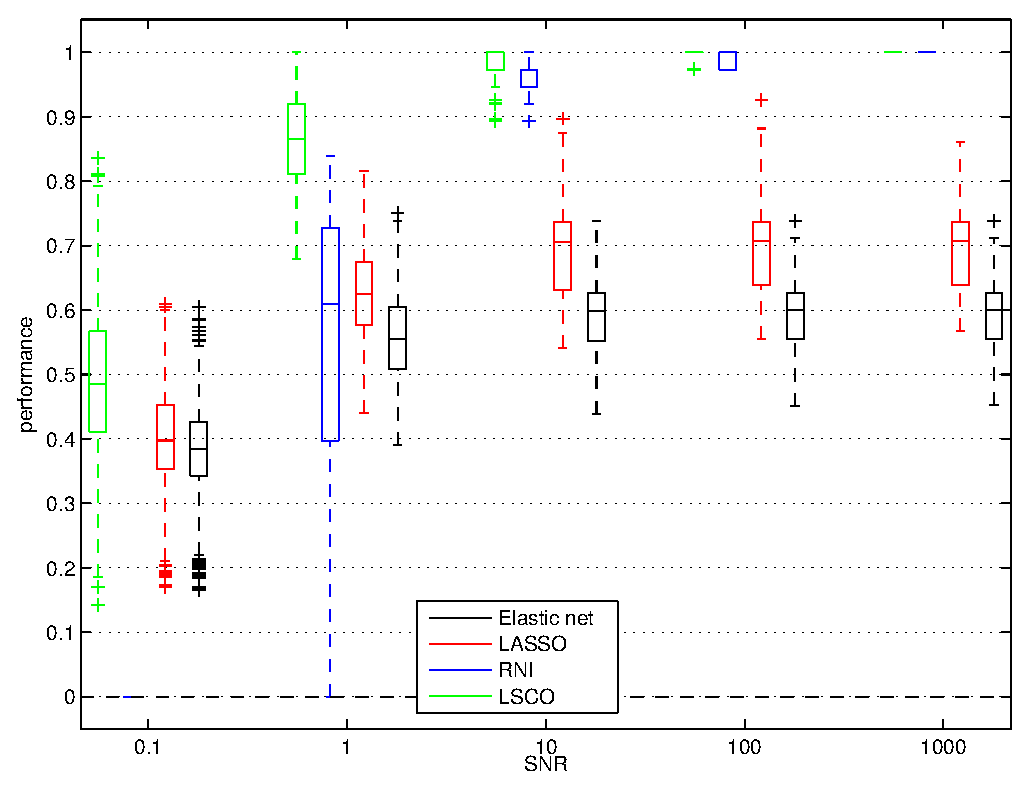
\includegraphics[width=1.0\linewidth]{./img/highkY_performance-nobkgr}
    \end{tikzfigure}
    \captionof{figure}{Performance on high $\kappa$ data sets as a
      function of the Signal to Noise Ratio\label{fig:highkY}}

    \begin{tikzfigure}{}
      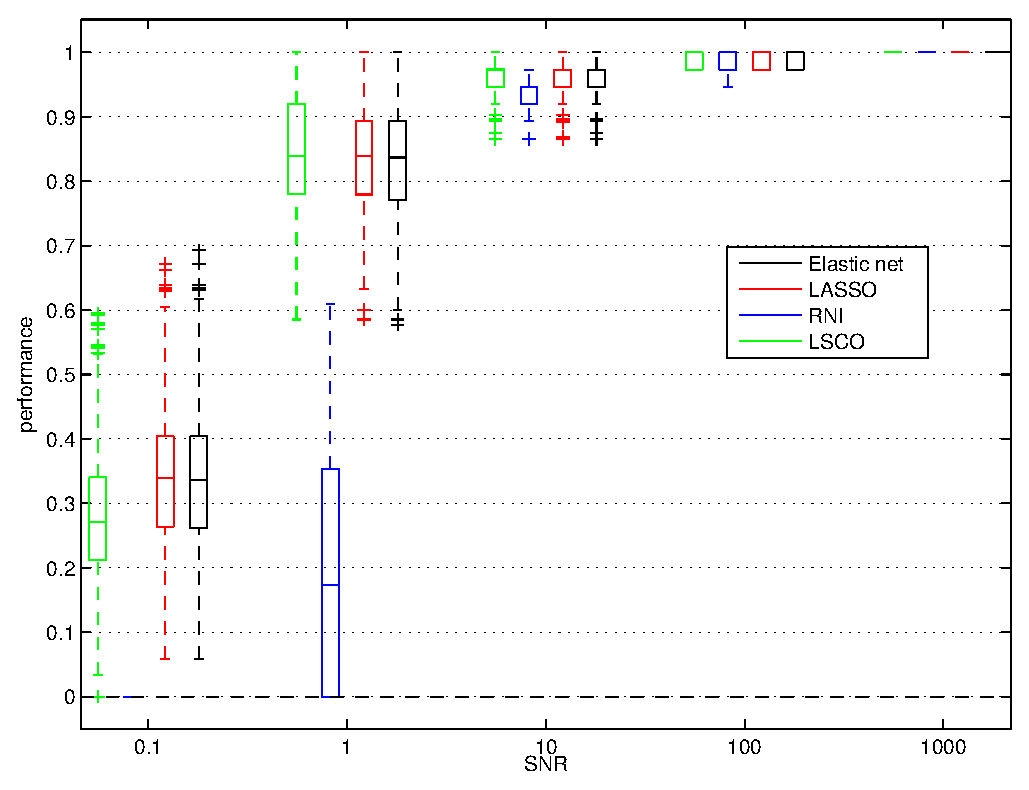
\includegraphics[width=1.0\linewidth]{./img/lowkY_performance-nobkgr}
    \end{tikzfigure}
    \captionof{figure}{Performance on low $\kappa$ data sets as a
      function of the Signal to Noise Ratio}
  }

  \column{0.3} \block{Discussion}{ The most striking result on the
    data set with high response matrix condition number is that
    all the $L_1$ regularisation methods fail to recover the true
    network model even when the SNR is so high that the data is
    informative enough for network inference and all existing
    links can be proven to exist
    \\\\
    The indicators SIC and WIC (Strong and Weak Irrepresentable
    Conditions) are fulfilled, only for the data sets with a low
    condition number and SNR of one or higher. An alternative
    representation of SIC can be seen in Figure
    \ref{fig:SIC-minRegDiff}.
    \\\\
    SIC and WIK cannot in practice be used to evaluate
    performance.  Until a better testable criterion for failure of
    $L_1$ regularisation is presented, we recommend all users to
    check the condition number of the response matrix. The
    condition number has the advantage of being a classical tool
    in linear algebra that is easy to calculate.

    \begin{tikzfigure}{}
      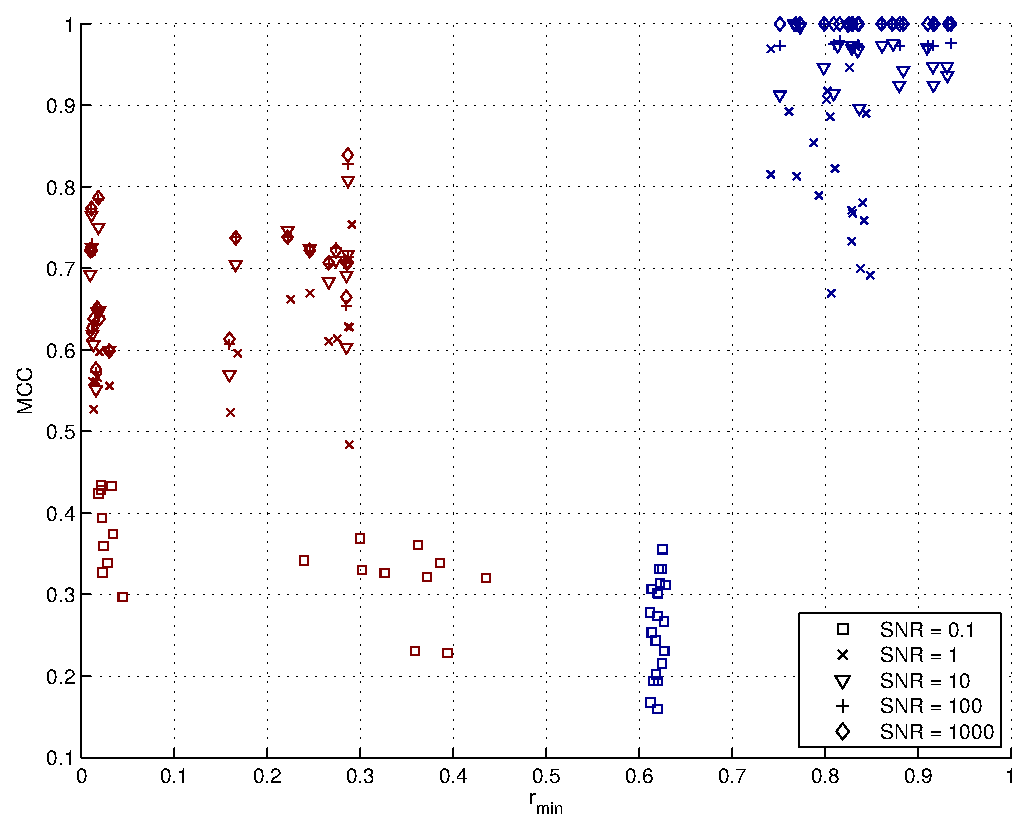
\includegraphics[width=1.0\linewidth]{./img/SIC-minRegDiff-nobkgr}
    \end{tikzfigure}
    \captionof{figure}{Performance of \lasso measured in $r_{min}
      =$ minimum ratio between the shortest regressor
      corresponding to a nonzero element and the longest
      corresponding to a zero.  Blue marks represent low $\kappa$
      data sets, while Red represents high $\kappa$ data sets. A
      clear separation is seen based on the condition number of
      the data\label{fig:SIC-minRegDiff}}
  }
\end{columns}

\begin{columns}
  \column{0.6}
  \block[titleoffsety=20mm,bodyoffsety=20mm]{Biological Data}{
    \begin{tabular}{l r}
      \begin{minipage}{0.7\linewidth}
        We demonstrate how our simulations can be used to
        estimate the optimal performance based on the properties
        of the ten gene network of the {Snf1} signalling pathway
        in \textit{S.\ cerevisiae} and the \invivo data collected
        by Lorenz \emph{et. al.}\cite{lorenz2009}. We identified
        the SNR $0.1$ data point in Figure \ref{fig:highkY} as the
        closest one in our simulations. We thus expect the optimal
        performance, in terms of MCC, of \lasso, Elastic Net,
        LSCO, and RNI to be far below $0.5$.
      \end{minipage}
      &
        \begin{tabular}{|l|rrr|}
          Performance & S10  & S19  & S9   \\
          \hline
          LASSO       & 0.18 & 0.22 & 0.36 \\
          LSCO        & 0.21 & 0.20 & 0.32 \\
          Elastic net & 0.18 & 0.27 & 0.40 \\
          NIR (S9)    & 0.25 & 0.28 & 1.00 \\
        \end{tabular}
    \end{tabular}
  }

     \note[targetoffsetx=-10cm,targetoffsety=-10cm,rotate=1,angle=10,width=.5\textwidth]{
       \bibliographystyle{plain}
       \bibliography{bibliography}
       }

  \column{0.4}
  \block[titleoffsety=-30mm,bodyoffsety=-30mm]{Conclusions}{
    \begin{itemize}
    \item $L_1$ regularisation methods--\lasso and Elastic
      Net--typically perform poorly in GRN inference when using
      data as ill-conditioned as typical experimental data.
    \item For both well-conditioned and ill-conditioned data, we
      found an SNR, of 10 to be sufficient for LSCO and RNI to
      achieve maximum accuracy close to one.
    \item For data with a SNR below one the accuracy of all
      methods was in general low.

    \end{itemize}

  }

\end{columns}

\end{document}


%%% Local Variables:
%%% TeX-master: "poster"
%%% ispell-local-dictionary: "en_GB"
%%% End:
